\documentclass{report}

\usepackage[latin1]{inputenc}
\usepackage[T1]{fontenc}
\usepackage[frenchb]{babel}
\usepackage[a4paper]{geometry}
\usepackage{lmodern}
\usepackage{listings}
\usepackage{color}
\usepackage{graphicx}
\usepackage{siunitx}
\usepackage{tikz}
\usepackage{pgfplots}
\usepackage{url}
\usepackage{amsmath, amsfonts}

\pgfplotsset{compat=newest}
\usepgfplotslibrary{units}

%definition des couleurs
\definecolor{newGreen}{rgb}{0,0.6,0}
\definecolor{newOrange}{rgb}{0.87,0.39,0.15}
\definecolor{newBlue}{rgb}{0.36,0.51,0.77}
\definecolor{newMauve}{rgb}{0.58,0,0.82}

\begin{document}
\renewcommand{\chaptername}{Partie}
	\begin{titlepage}
		\vspace{-10px}
		\begin{tabular}{l}
			\textsc{Blin} S\'ebastien, \\
			\textsc{Collin} Pierre-Henri, \\
			\textsc{Louarn} Amaury 
		\end{tabular}
		\hfill \vspace{10px}
\includegraphics[scale=0.15]{ur1.png}\\
		\vfill
		\begin{center}
			\Huge{Universit\'e de Rennes 1}\\
			\large{Campus de Beaulieu}\\
			\vspace{1cm}
			\LARGE{Licence STS}\\
			\large{Cycle Pr\'eparatoire Ing\'enieur Rennes 1 - Informatique et T\'el\'ecommunications}\\
			\vspace{0.5cm}\hrule\vspace{0.5cm}
			\LARGE{\textbf{Rapport de Travail d'Initiative Personnelle Encadr\'ee (TIPE)}}\\
			\Large{Comment la reconnaissance faciale du conducteur peut-elle am\'eliorer sa s\'ecurit\'e au volant ?}
			\vfill
			\vfill
		\end{center}
		\begin{flushleft}
			\Large{Sous l'encadrement de~:}\\
			\vspace{0.2cm}
			\large{Johanne B\'ezy-Wendling}\\
			\normalsize{Ma\^itre de Conf\'erences\\
			Responsable cycle pr\'eparatoire ing\'enieur de l'Universit\'e de Rennes I\\
			(sp\'ecialit\'e informatique et t\'el\'ecommunications)}\\
			\vspace{0.2cm}
			\large{Finn J\o rgensen}\\
			\normalsize{Responsable L3 d'informatique - ISTIC}
		\end{flushleft}
		\vfill
	\end{titlepage}
	\begin{abstract}
		%TODO
	\end{abstract}
	\chapter*{Introduction}
		\subsection*{Pourquoi ce projet}
			%TODO
	\chapter{Les limites de la s\'ecurit\'e routi\`ere}
		Dans cette premi\`ere partie, nous allons aborder les limites de la s\'ecurit\'e routi\`ere, qui sont \`a l'origine de notre probl\'ematique. D'abord, nous verrons les moyens mis en oeuvre pour prot\'eger l'automobiliste. Puis, nous verrons les comportements \`a risque qui nuisent encore \`a sa s\'ecurit\'e.
		\section{Les moyens mis en place pour la s\'ecurit\'e du conducteur en France.}
			Dans le but de visualiser les moyens d\'eploy\'es par les pouvoirs publics, nous ferons dans un premier temps un historique de la s\'ecurit\'e routi\`ere depuis le d\'ebut des ann\'ees 70 (p\'eriode qui correspond \`a l'adoption des premi\`eres mesures pour diminuer le nombre de morts sur la route). Ensuite, nous verrons l'impact induit par ces moyens sur l'augmentation de la s\'ecurit\'e au volant.
			\subsection{Historique de la s\'ecurit\'e routi\`ere depuis 40 ans}

Apr\`es la seconde guerre mondiale, et en particulier d\`es le d\'ebut des ann\'ees 50, le nombre d'accidents mortels sur la route a fortement augment\'e. Plusieurs facteurs sont en cause~: l'expansion du parc automobile, un r\'eseau routier inadapt\'e, ainsi que l'insuffisante formation des conducteurs. Le premier d\'enombrement en 1954 recensa 7166 tu\'es en 3 jours. \`a cette \'epoque, la s\'ecurit\'e routi\`ere \'etait de loin un probl\`eme prioritaire pour le gouvernement car il n'y avait pas encore de politique publique.\\

\`a partir des ann\'ees 60, ce fut le d\'ebut des op\'erations de traitement des points noirs \#\#(peut-�tre des pr\'ecisions \`a apporter mais pas encore trouv\'e)\#\#. Entre 1960 entre 1970, la mortalit\'e augmenta de 55,7\% et le trafic est multipli\'e par 2,3.\\

En 1972, le Comit\'e Interminist\'eriel de la S\'ecurit\'e Routi\`ere (C.I.S.R) fut cr\'e\'e afin de d\'efinir la politique de s\'ecurit\'e routi\`ere en France. Cette ann\'ee fut aussi celle qui aura fait le plus de victimes sur les routes avec 16 545 morts. Durant la d\'ecennie qui suivie, le gouvernement instaura plusieurs mesures telles que~: les limitations de vitesse et l'obligation du port de la ceinture \`a l'avant. En dix ans, la mortalit\'e diminua de 30\% tandis que le trafic global fut multipli\'e par 1,6.\\

Au d\'ebut des ann\'ees 80, les pouvoirs publics constat\`erent une stabilisation de la baisse de la mortalit\'e routi\`ere. Ils instaur\`erent des plans d\'epartementaux de s\'ecurit\'e routi\`ere ainsi que le programme R.E.A.G.I.R (R\'eagir pour les Enqu�tes sur les Accidents Graves et les Initiatives pour y Rem\'edier). Ce fut \'egalement le d\'ebut de la politique locale de s\'ecurit\'e routi\`ere. Entre 1980 et 1990, le seuil d'alcool\'emie autoris\'e fut abaiss\'e de 1,2 \`a 0,8 g/l d'alcool dans le sang, la plupart des v\'ehicules furent \'equip\'es d'un syst\`eme anti-blocage des roues, le nombre de carrefours giratoires augmenta (diminution notable du nombre d'accidents mortels dans les carrefours).\\

\`a la fin des ann\'ees 80, un livre blanc de la s\'ecurit\'e routi\`ere fut publi\'e dans le but d'\'enoncer les orientations majeures des futures politiques de s\'ecurit\'e routi\`ere. Entre 1990 et 2000, de nombreuses mesures furent donc mises en oeuvre~: en 1990, la vitesse maximale autoris\'ee en agglom\'eration fut fix\'ee \`a 50km/h et un permis \`a points fut instaur\'e, le taux d'alcool autoris\'e dans le sang se limita \`a 0,5 g/l, l'essentiel du r\'eseau autoroutier \'etait quasiment achev\'e, la plupart des v\'ehicules furent \'equip\'es d'airbags. De plus, le continuum \'educatif est mis en place. D'apr\`es le site gouvernemental de la s\'ecurit\'e routi\`ere, le continuum \'educatif exprima l'id\'ee que "l'\'education \`a la s\'ecurit\'e routi\`ere ne se fait pas seulement lors du passage du permis de conduire, mais tout au long de sa vie".\\
En dix ans, le trafic global augmenta de 20\%, alors que la mortalit\'e routi\`ere diminua d'autant.\\

En 2002, la s\'ecurit\'e routi\`ere \'etait l'un des principaux chantiers du Pr\'esident de la R\'epublique. Un an plus tard, les premiers radars de contr�le/sanction automatiques //--syst\`emes de sanction automatique--// arriv\`erent au bord des routes. La m�me ann\'ee, le Conseil National de la S\'ecurit\'e Routi\`ere (C.N.S.R) s'installa \#\#pr\'eciser ses missions\#\#. En 2004, le permis probatoire fit son apparition. Les sanctions sont devenues plus importantes pour les conducteurs en \'etat d'\'ebri\'et\'e. En effet, un d\'epassement du taux l\'egal d'alcool dans le sang entraine un retrait de six points sur le permis de conduire. En 2000 et 2010, la mortalit\'e baissa de 51,1\% alors que le trafic global augmenta de 7\%.\\

Apr\`es un bref aper�u sur l'\'etendu des d\'ecisions prises par les gouvernements depuis 1972 en mati\`ere de s\'ecurit\'e routi\`ere, nous allons maintenant voir quel est le bilan de ces mesures.\\

\subsection{Bilan de quarante ann\'ees de mesures}

Premi\`erement, le nombre de tu\'es sur la route a fortement diminu\'e depuis 1972 (ann\'ee qui marque la fin de la hausse constante de la mortalit\'e routi\`ere). Comme nous pouvons le constater sur le graphique ci-dessus/ci-dessous, ce nombre a \'et\'e divis\'e par plus de quatre en quarante ans malgr\'e un doublement du parc automobile. En 2012, 3 653 personnes ont \'et\'e tu\'ees en 30 jours contre plus de 18 000 en 1972.\\

\begin{figure}
	\begin{center}
		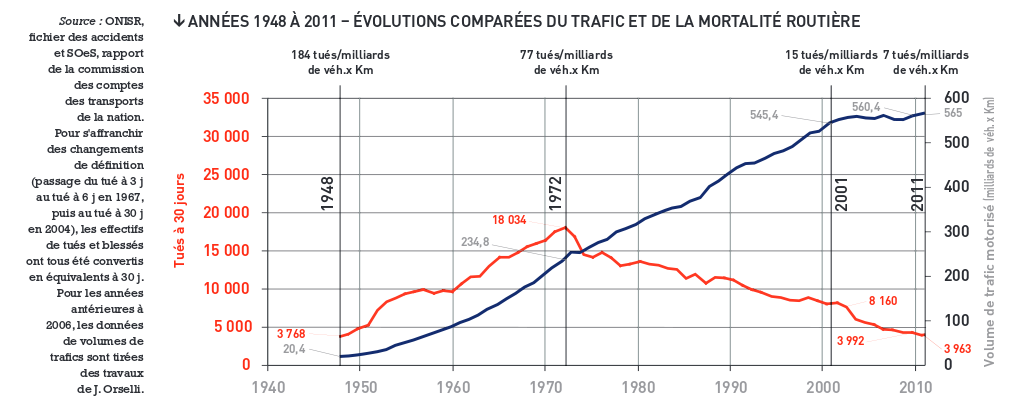
\includegraphics[scale=0.41]{images/evolcompart48-11.png}
		\caption{\'Evolution compar\'ee du traffic et de la mortalit\'e routi\`ere entre 1948 et 2011}
	\end{center}
\end{figure}

Ces progr\`es observ\'es en mati\`ere de s\'ecurit\'e routi\`ere ont \'et\'e obtenus en agissant sur plusieurs facteurs. Lors d'un accident, quatre facteurs essentiels doivent �tre pris en compte~: tout d'abord les facteurs li\'es \`a l'infrastructure (conception, entretien et exploitation), les facteurs li\'es aux v\'ehicules (s\'ecurit\'e passive et active), les facteurs li\'es aux comportements des usagers (formation, communication, r\'epression), et le progr\`es des services de secours et de soin. Cependant, il est tr\`es difficile de d\'efinir la part de chacun de ces facteurs dans l'am\'elioration de la s\'ecurit\'e routi\`ere. \\

Concernant les facteurs li\'es \`a l'infrastructure, nous pouvons retenir plusieurs points qui ont particip\'e \`a l'am\'elioration de la s\'ecurit\'e routi\`ere~: comme la construction d'un r\'eseau autoroutier, le d\'eploiement de barri\`eres de s\'ecurit\'e le long des routes potentiellement dangereuses, les protections anti-\'eblouissements, des bandes sonores anti-endormissement, les bandes d'arr�ts d'urgences. \\

Ensuite parmi les facteurs li\'es aux v\'ehicules, la situation actuelle n'a plus rien \`a voir avec celle d'il y a quarante ans. Le port obligatoire de la ceinture, l'obligation pour les enfants de s'asseoir \`a l'arri\`ere du v\'ehicule, l'apparition de diff\'erents coussins gonflables de s\'ecurit\'e dans le poste conducteur (airbags), la structure des v\'ehicules qui absorbent mieux les chocs (\`a l'aide des pare-chocs par exemple) ont eu un impact consid\'erable sur la diminution de la gravit\'e des accidents. Nous pouvons aussi \'evoquer la mise en place progressive dans tous les v\'ehicules de syst\`emes d'aide \`a la conduite (ABS par exemple). \\

Les facteurs li\'es aux comportements des usagers sont s�rement ceux qui ont eu le plus d'effets sur la diminution du nombre de tu\'es sur la route. Tout d'abord, la formation des usagers qui n'a cess\'e de cro\^itre au fil des ann\'ees a permis de leur donner une meilleure appr\'ehension de la route. Cette formation s'inscrit dans un processus progressif et continu. Que ce soit en famille, \`a l'\'ecole, lors du passage du permis de conduire, ou pendant le reste de leur vie. Ensuite, la r\'epression a incit\'e les usagers \`a respecter les nouvelles mesures de s\'ecurit\'e mises en place. Par exemple, sur le respect des limitations de vitesse, du taux d'alcool\'emie pr\'esent dans le sang, du port de la ceinture, etc. Au fil du temps, la r\'epression s'est durcie avec l'augmentation des points retir\'es en cas de d\'elit. Enfin, la communication sur la s\'ecurit\'e routi\`ere a \'et\'e primordiale pour faire changer les moeurs.
Des campagnes publicitaires (voir ci-dessous) parfois chocs ont fait prendre conscience aux usagers que nous sommes "tous responsables" (slogan utilis\'e lors des campagnes de pr\'evention).\\

\begin{figure}
	\begin{center}
		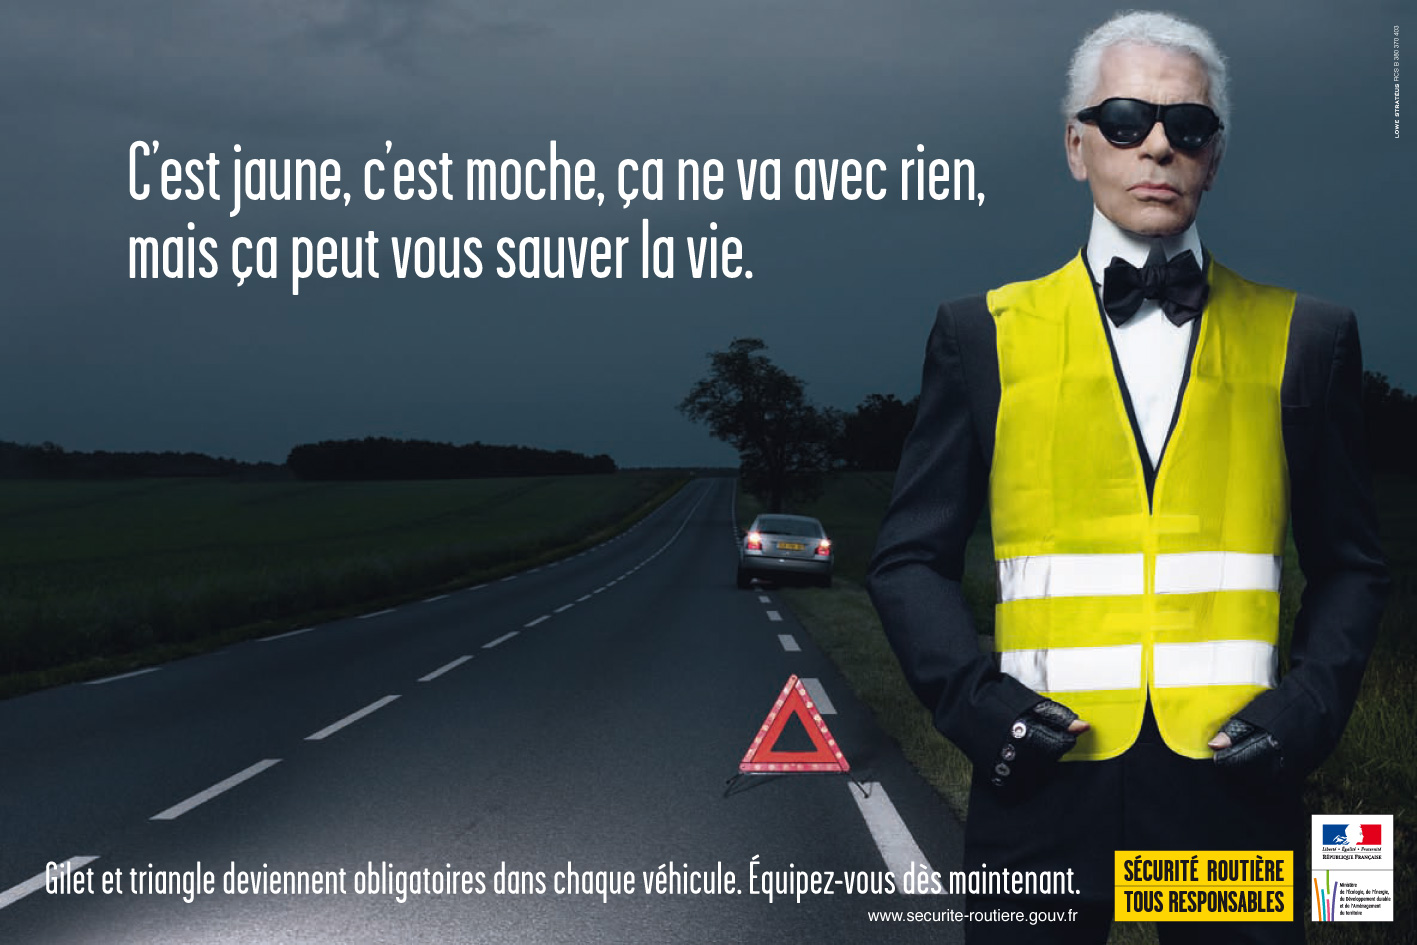
\includegraphics[scale=0.25]{images/karl-for-Securite-Routiere}
		\caption{Karl Lagarfeld pour une affiche de pr\'eventions routi\`ere}
	\end{center}
\end{figure}
 
Suite \`a cette pr\'esentation des moyens mis en oeuvre par les gouvernements successifs et de leurs impacts sur la s\'ecurit\'e routi\`ere, nous allons \`a pr\'esent aborder les limites de ces mesures, c'est-\`a-dire les comportements qui mettent en p\'eril cette s\'ecurit\'e.\\

\section{Les comportements \`a risques}

Malgr\'e toutes les mesures prises pour prot\'eger le conducteur, de nombreux accidents mortels ont encore lieu. La plupart du temps, cet accident n'est pas d� \`a une d\'efaillance du v\'ehicule, une route endommag\'ee ou encore au mauvais temps, mais \`a une d\'efaillance humaine. C'est pourquoi, nous analyserons d'abord les principales causes des accidents, puis un type de comportement dangereux en particulier~: la conduite \`a l'aveugle.

\subsection{Les principales causes d'accidents}

Les accidents corporels sont g\'en\'eralement d\'etermin\'es par plusieurs facteurs.Ces facteurs peuvent influer sur l'occurrence des accidents, mais aussi sur leur gravit\'e. Ils sont souvent li\'es entre eux, et il est particuli\`erement difficile de d\'eterminer le facteur principal, habituellement appel\'e la "cause" de l'accident.\\

La vitesse est un facteur pr\'epond\'erant dans les accidents corporels. C'est \'egalement un facteur transversal, car la vitesse est presque toujours pr\'esente comme facteur d'occurrence et/ou facteur de gravit\'e. En 2011, en France, au moins 26\% des accidents mortels ont pour cause identifi\'ee la vitesse d'apr\`es les forces de l'ordre. En Suisse et en Allemagne la vitesse, seule ou associ\'ee, repr\'esente 40\% des accidents mortels.\\

L 'alcool est \'egalement un facteur majeur pr\'esent dans les accidents. En effet, s'il est pr\'esent dans le sang en quantit\'e trop importante, il entra\^ine une augmentation de la vitesse, la somnolence, l'oubli du port de la ceinture de s\'ecurit\'e. Le taux d'implication de l'alcool dans la mortalit\'e routi\`ere reste constant~: environ 31\%.Les 875 accidents mortels avec au moins un conducteur ayant une alcool\'emie sup\'erieur au seuil autoris\'e ont provoqu\'e 964 victimes. Parmi les victimes des accidents mortels avec comme facteur l'alcool, les conducteurs ainsi que leurs passagers repr\'esentent 70\% des personnes tu\'ees.\\

Les autres facteurs sont~:
\begin{itemize}
	\item{L'usage des stup\'efiants (en 2011, 455 accidents mortels avec au moins un conducteur test\'e positivement aux stup\'efiants). Ces accidents ont entrain\'es le d\'ec\`es de 499 personnes (soit 13\% de la mortalit\'e routi\`ere).}
	\item{La prise de m\'edicaments~: une \'etude r\'ealis\'ee par une \'equipe de l'INSERM (projet CESIR-A) a montr\'e que 3\% des accidents \'etaient attribuables \`a la prise de produits m\'edicamenteux.}
	\item{le respect des distances de s\'ecurit\'e. D'apr\`es le Code de la Route~: \og Lorsque deux v\'ehicules se suivent, le conducteur du second doit maintenir une distance de s\'ecurit\'e suffisante pour pouvoir \'eviter une collision en cas de ralentissement brusque ou d'arr�t subit du v\'ehicule qui le pr\'ec\`ede. Cette distance est d'autant plus grande que la vitesse est plus \'elev\'ee. Elle correspond \`a la distance parcourue par le v\'ehicule pendant un d\'elai d'au moins deux secondes\fg. Globalement, plus de 50\% des conducteurs ne respectent pas cette r\`egle. Or, le non-respect des distances de s\'ecurit\'e qui entrainent des collisions par l'arri\`ere et des collisions en chaine totalise 6.2\% de la mortalit\'e routi\`ere.}
	\item{Le port de la ceinture~: en 2011, 22\% des personnes tu\'ees n'\'etaient pas ceintur\'ees.}\\
\end{itemize}

Comme nous venons de le voir, les principales causes d'accidents mettent en avant le comportement de l'usager. Nous allons nous attarder sur une une cause d'accident qui n'a pas \'et\'e \'evoqu\'ee pr\'ec\'edemment~: la distraction du conducteur.\\

\subsection{La conduite \`a l'aveugle}

La conduite \`a l'aveugle fait r\'ef\'erence au rel�chement d'attention du conducteur pour effectuer d'autres t�ches annexes \`a l'int\'erieur du v\'ehicule. Ainsi, ses capacit\'es d'analyse de la circulation et de r\'eaction sont fortement diminu\'ees.\\

Il existe trois types de distraction~: visuelle (regarder autre chose que la route), manuelle (d\'etacher ses mains du volant), cognitive (ne pas �tre concentr\'e sur la route). Concr\`etement, cela signifie~: utiliser sont t\'el\'ephone portable ou un smartphone, envoyer un sms, manger et boire, parler aux passagers, se maquiller, lire (y compris les cartes), utiliser un syst\`eme de navigation, regarder une vid\'eo, r\'egler la radio, un lecteur CD ou mp3, etc. Envoyer des sms est la distraction la plus dangereuse, car elle combine les trois types de distraction. De plus, envoyer ou lire un texte oblige \`a quitter des yeux la route pendant 4,6 s en moyenne. A 55 mph (environ 88 km/s), c'est comme conduire la longueur d'un terrain de football, les yeux band\'es.\\

En France, certaines \'etudes ont montr\'e que 25\% \`a 50\% des accidents corporels \'etaient dus \`a la distraction du conducteur. A l'\'etranger, la conduite \`a l'aveugle est \'egalement un facteur de plus en plus important dans la mortalit\'e routi\`ere. Par exemple, chaque jour aux Etats-Unis, plus de 9 personnes sont tu\'ees et plus de 1,060 personnes sont bless\'ees dans des accidents o\`u sont impliqu\'es un conducteur distrait. Par ailleurs, beaucoup d'usagers (en particuliers les jeunes) ne semblent pas encore avoir pris conscience du danger de ces pratiques. En effet, d'apr\`es un sondage r\'ealis\'e en 2011 aux Etats-Unis, 69\% des conducteurs �g\'es de 18 \`a 64 ans avaient t\'el\'ephon\'e en conduisant (En Europe, ce taux varie entre 21\% au Royaume-Uni \`a 59\% au Portugal) et 31\% avaient lu ou envoy\'es un sms en conduisant dans les 30 derniers jours avant d'�tre sond\'es.\\

	\chapter{La reconnaissance faciale}
		Dans cette deuxieme partie, nous nous pencherons sur la reconnaissance faciale. Dans un premier temps, nous \'etudierons l'aspect th\'eorique de la reconnaissance, puis  l'aspect exp\'erimental.

\section{Th\'eorie}

Afin d'\'etudier l'aspect th\'eorique de la reconnaissance faciale, nous allons d'abord l'aborder de fa�on g\'en\'eral. Ensuite, nous analyserons plus en d\'etail diff\'erentes m\'ethodes de reconnaissance~: Eighenface, Fisherface et LBPH.

\subsection{G\'en\'eralit\'es}

Apr\`es des recherches approfondies, nous avons pu constater qu'il existe \'enorm\'ement de m\'ethodes possibles pour reconna�tre un visage.  Ces m\'ethodes peuvent \'egalement �tre combin\'ees entre elles (par exemple, la mise en place en place d'un r\'eseau neuronal \#\#explication peut-�tre ?\#\#). Cependant, en trois mois, nous nous n'aurions pas eu le temps de mettre en place une telle m\'ethode.\\

Par ailleurs, nous avons choisi de traiter uniquement des images en noir et blanc, car la colorim\'etrie a tr\`es peu d'impact dans le processus de reconnaissance.\\

\subsection{La m\'ethode Eighenface}

La m\'ethode de reconnaissance faciale Eighenface a pour particularit\'e de se baser sur des \og eighen vectors\fg, c'est-\`a-dire des vecteurs propres. Elle a \'et\'e introduite en 1991 par Turk et Pentland\\

L'algorithme est le suivant~: chaque image est consid\'er\'ee comme un vecteur avec pour dimension son nombre de pixels. Puis, un ou plusieurs algorithmes recherchent les principales composantes //--plus de pr\'ecision sur composante ?--//. A l'aide de plusieurs images du m�me visage, nous pouvons alors composer une image du visage \og moyen\fg qui contiendra \'egalement les principales composantes (l'eighenface). La m\'ethode de reconnaissance des axes principaux est d\'etaill\'ee ici~: Matthew Turk and Alex Pentland. Eigenfaces for recognition. J. Cognitive Neuroscience. 3(1)~:71{86, 1991}. Enfin, il suffit de comparer l'eighenface et les composantes principales d'une capture d'un visage.\\

L'avantage de cette m\'ethode est la connaissance de son existence depuis longtemps. Cependant, elle pr\'esente \'egalement des d\'esavantages non-n\'egligeables. En effet, comme chaque pixel est une dimension, une image $100\times100$ donne 10000 vecteurs \`a traiter. Le nombre de donn\'ees \`a analyser est donc trop important.\\

\subsection{La m\'ethode Fisherface}

La m\'ethode de reconnaissance faciale Fisherface se base sur les travaux de Sir R.A. Fisher. L'id\'ee de base de l'algorithme est la suivante~: toutes les images qui se ressemblent, se retrouvent proches. Concr\`etement, imaginons un espace d'images comprenant une \'echelle repr\'esentant les visages. Si nous projetons les images sur l'\'echelle, nous pouvons dire que //-- je n'ai pas compris la suite --//\\

\begin{figure}[h]
	\begin{center}
		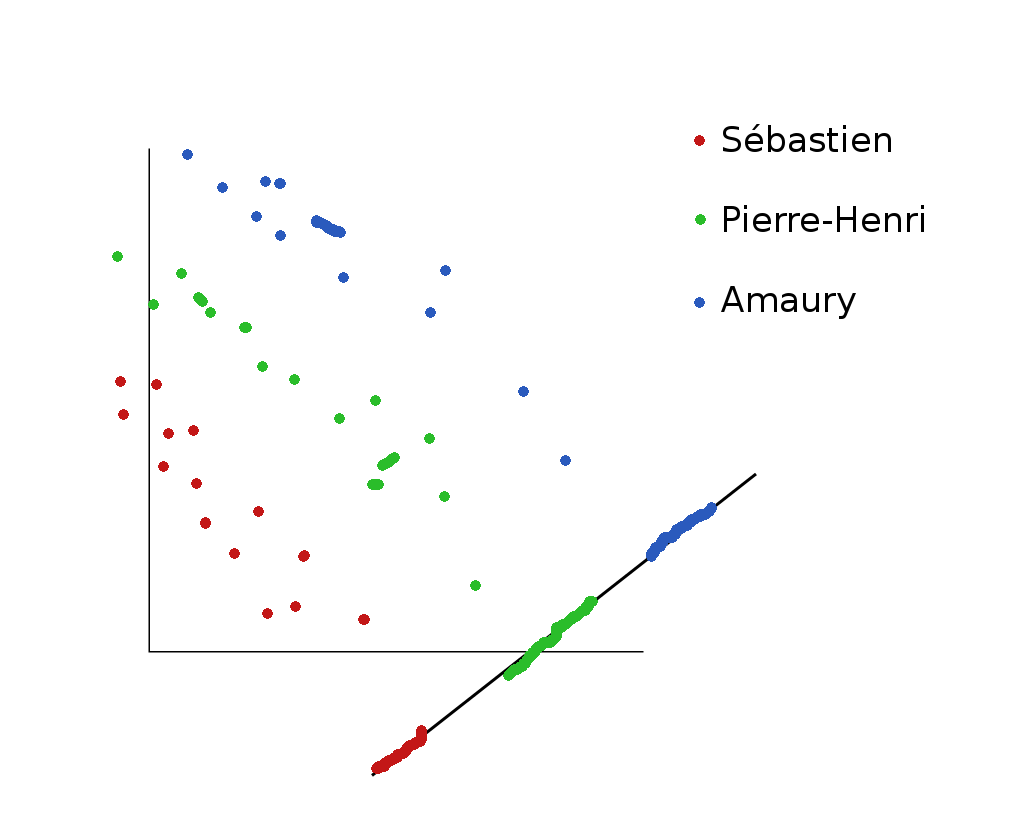
\includegraphics[scale=0.3]{images/fisherfacedistrib.png}
		\caption{Distribution Fisherface}
	\end{center}
\end{figure}

Pour plus de d\'etails~: \url{http://docs.opencv.org/modules/contrib/doc/facerec/facerec_tutorial.html#fisherfaces}.\\

Globalement, cette m\'ethode pr\'esente les m�mes avantages et inconv\'enients que la m\'ethode Eighenface. Cependant, elle est moins sensible \`a la lumi\`ere et \`a la d\'eformation des visages car elle ne se base pas sur des composantes discriminatoires.\\

\subsection{La m\'ethode LBPH}

La m\'ethode de reconnaissance faciale LBPH (Local Binary Patterns Histogram) consiste \`a visualiser la valeur d'un pixel (moyenne des trois composantes RGB) par rapport aux pixels voisins.\\

Pour commencer, l'image est divis\'e en groupe de pixels. Chaque groupe de pixels correspond \`a une matrice carr\'e contenant les valeurs des pixels. Puis, le pixel plac\'e au centre de la matrice est choisi comme valeur de r\'ef\'erence. Ensuite, toutes les valeurs de la matrice sont remplac\'ees soit par 0, soit par 1 en fonction de leur valeur. La fonction d'Heaviside, nous dit que 
\[
	\forall x \in \mathbb{R}, H(x)=
	\left \{
	\begin{array}{l l}
		0 & \text{si } x \leq 0\\
		1 & \text{sinon}
	\end{array}
	\right.
\]
Ici, si nous attribuons la valeur 0 si la valeur du pixel est inf\'erieur \`a la valeur du pixel de r\'ef\'erence, 1 sinon. Apr\`es cette op\'eration, chaque pixel du groupe est pond\'er\'e avec un poids plus ou moins fort (le pixel en haut \`a gauche a le poids le plus faible, tandis que le pixel en bas \`a droite a le poids le plus fort). Ainsi, nous obtenons un nombre binaire qui donne une certaine valeur en base 10. Tous les groupes de l'image sont soumis \`a ce processus pour finalement obtenir un histogramme de l'image. Enfin, il ne reste plus qu'\`a faire la diff\'erence entre deux histogrammes pour comparer deux images.\\

Cet algorithme est tr\`es utilis\'e comme nous pouvons le voir dans~: Facial expression recognition based on Local Binary Patterns:A comprehensive study de Caifeng Shan a, * , Shaogang Gong b , Peter W. McOwan b, o\`u il est combin\'e avec Adaboost (plugin d'openCV) pour obtenir de meilleurs r\'esultats, et un r\'eseau neuronnal. Mais aussi dans~: Face Recognition with Local Binary Patterns, Spatial Pyramid Histograms and Naive Bayes Nearest Neighbor (NBNN) classification de Daniel Maturana, Domingo Mery and Alvaro Soto o\`u les auteurs essayent d'am\'eliorer l'algorithme dans le but d'en cr\'eer un nouveau~: NBNN. Nous n'utiliserons pas cet algorithme par manque de temps, mais \'egalement car LBPH est d\'ej\`a pr\'esent dans openCV.\\

Comme nous venons de le voir, il existe diff\'erents m\'ethodes 

\section{Exp\'erimentations}
Dans cette partie, nous exp\'erimenterons les m\'ethodes de reconnaissance de visage \'evoqu\'ees dans la premi\`ere partie. D'abord, nous verrons le protocole exp\'erimental, puis la r\'ealisation des exp\'eriences et enfin, les r\'esultats et analyses de ces manipulations.
\subsection{Protocole}
Le but de l'exp\'erimentation \'etait de comparer les trois m\'ethodes (Eigenface, Fisherface et LBPH) impl\'ement\'ees par la librairie OpenCV de fa�on \`a en choisir une pour notre application finale, puis d'\'etudier sa robustesse. Nous avons r\'ealis\'e deux exp\'eriences : la premi\`ere consistait \`a observer la vitesse de reconnaissance en fonction du nombre d'images pr\'esentes dans la base de donn\'ees et de comparer le pourcentage de r\'eussite. La seconde exp\'erience cherchait \`a \'etudier la robustesse de la m\'ethode, c'est-\`a-dire si elle marchait \'egalement pour des cas particuliers comme un visage partiellement cach\'e ou quand l'utilisateur r\'ealisait grimace.
\subsection{R\'ealisation des exp\'eriences}
Lors de la premi\`ere exp\'erience, nous avons mesur\'e deux vitesses d'ex\'ecution : le temps d'importation des images pour r\'ealiser l'entrainement de l'algorithme et l'entrainement de l'algorithme (premier temps) et le temps pour r\'ealiser la reconnaissance (second temps). La base de donn\'ees \'etait compos\'ee de trois individus. Nous avons d'abord captur\'e une photo d'un des individus pr\'esents dans la base. Nous avons ensuite utilis\'ee cette photo pour tester les trois algorithmes (Eigenface, Fisherface et LBPH). Pour chaque m\'ethode, l'op\'eration a \'et\'e r\'ep\'et\'ee cent fois sur le m�me ordinateur (afin d'\'eviter les impr\'ecisions dues au processeur qui ne travaille pas toujours de mani\`ere identique). Nous avons \'egalement vari\'e le nombre de photos pr\'esentes dans la base de donn\'ees : 1, 2, 4, 6, 8, 10, puis 12 photos par individu. \\

Dans la deuxi\`eme partie de l'exp\'erience, nous avons pris une vid\'eo compos\'ee de cent images pendant laquelle le sujet bougeait doucement la t�te dans toutes les directions. Par ailleurs, chaque sujet \'etait enregistr\'e dans la base de donn\'ees \`a l'aide de douze photos prises dans diff\'erentes postures. Pour finir, chaque algorithme \'etait appliqu\'e aux cent images de la vid\'eo pour observer le pourcentage de r\'eussite.\\

Pour la seconde exp\'erience qui cherche \`a \'etudier la robustesse d'un algorithme, nous avons privil\'egi\'e la m\'ethode LBPH qui montrait de meilleurs r\'esultats lors de notre premi\`ere exp\'erience. Nous avons demand\'e \`a plusieurs personnes de s'enregistrer dans la base de donn\'ees. Ensuite, pour chacune de ces personnes, une vid\'eo compos\'ee de 100 images a \'et\'e prise. Par ailleurs, les sujets ont \'et\'e film\'ees sous diff\'erentes conditions. Nous avons vari\'e la luminosit\'e (faible, naturelle, \'elev\'ee), l'orientation et l'inclinaison de la t�te. Nous avons aussi accentu\'e la d\'eformation du visage, cach\'e certaines parties du visage et modifi\'e la distance par rapport \`a la cam\'era. La cam\'era utilis\'ee \'etait la m�me que celle utilis\'ee lors de l'enregistrement de l'individu dans la base de donn\'ees pour \'eviter tout changement de r\'esolution possible.
\subsection{R\'esultats et analyses}
Concernant l'exp\'erience \no 1, l'algorithme Fisherface a \'et\'e le plus rapide dans l'\'elaboration du mod\`ele, suivi par Eigenface puis LBPH (voir Figure~\ref{fig:dureesAlgos}). Nous pouvons noter qu'Eigenface devient de plus en plus lent \`a mesure que le nombre d'images dans la base de donn\'ees augmente (au bout de 36 images, la m\'ethode est aussi lente que LBPH). \\
\begin{figure}[h]
	\begin{center}
	\begin{tikzpicture}
		\begin{axis}[
			width=5.9cm,
			height=5cm,
			xlabel={nombre d'images dans la base de donn\'ee},
			ylabel={temps d'ajout},
			y unit=\si{\second}
		]
			\addplot  table[x=nb,y=tps,col sep=comma] {data/ByNumberOfImages_rec_eigenface.csv};
			\addplot  table[x=nb,y=tps,col sep=comma] {data/ByNumberOfImages_rec_fisherface.csv};
			\addplot  table[x=nb,y=tps,col sep=comma] {data/ByNumberOfImages_rec_LBPH.csv};
		\end{axis}
	\end{tikzpicture}
	\begin{tikzpicture}
		\begin{axis}[
			width=5.9cm,
			height=5cm,
			xlabel={nombre d'images dans la base de donn\'ee},
			ylabel={temps de reconnaissance},
			y unit=\si{\second},
			 legend style={at={(0.9,0.5)},anchor=west},
			legend entries={eigenface,fisher face,LBPH}
		]
			\addplot  table[x=nb,y=tps,col sep=comma] {data/ByNumberOfImages_bdd_eigenface.csv};
			\addplot  table[x=nb,y=tps,col sep=comma] {data/ByNumberOfImages_bdd_fisherface.csv};
			\addplot  table[x=nb,y=tps,col sep=comma] {data/ByNumberOfImages_bdd_LBPH.csv};
		\end{axis}
	\end{tikzpicture}
	\caption{Dur\'ees d'initialisation, et de reconnaissance, par algorithme}
	\label{fig:dureesAlgos}
	\end{center}
\end{figure}
Pour la reconnaissance des visages, la dur\'ee est quasiment identique pour les trois algorithmes. Elle est comprise entre 680 et 690 ms pour un processeur Intel Core i5 de deuxi\`eme g\'en\'eration. Nous pouvons donc conclure que le temps n'est pas un facteur important dans le choix de l'algorithme. Si nous choisissons de prendre LBPH, l'initialisation prendra plus le temps, mais il n'y aura pas d'impact sur le temps de reconnaissance.

\begin{figure}[t]
	\begin{center}
	\begin{tikzpicture}
		\begin{axis}[
			xbar,
			xmin=0,
			width=12cm,
			height=8cm,
			enlarge y limits=0.15,
			xlabel={Pourcentage de reconnaissance},
			symbolic y coords={Moyenne, {}, Amaury, Pierre-Henri, S\'ebastien},
			ytick=data,
			nodes near coords,
			nodes near coords align={horizontal},
			legend style={at={(0.5,0.36)},anchor=north,legend columns=-1},
		]
			\addplot coordinates {(71.929824561404,Amaury) (7.4074074074074,Pierre-Henri) (24.657534246575,S\'ebastien) (34.6649220717955,Moyenne)};
			\addplot coordinates {(59.649122807018,Amaury) (80.246913580247,Pierre-Henri) (73.972602739726,S\'ebastien) (71.2895463756637,Moyenne)};
			\addplot coordinates {(82.456140350877,Amaury) (60.493827160494,Pierre-Henri) (90.41095890411,S\'ebastien) (77.786975471827,Moyenne)};
			
			\legend{Eigenface, Fisherface, LBPH}
		\end{axis}
	\end{tikzpicture}
	\caption{Pourcentage de reconnaissance, en fonction du cobaye et de l'algorithme}
	\label{fig:pourcentageReco}
	\end{center}
\end{figure}
Nous d\'eduisons de la seconde partie de l'exp\'erience \no 1 les r\'esultats affich\'es Figure~\ref{fig:pourcentageReco}. Nous remarquons que l'algorithme LBPH est globalement meilleur que les deux autres. Fisherface arrive deuxi\`eme, suivi de loin par Eigenface.\\

Nous pouvons conclure de la seconde partie que la luminosit\'e peut �tre un probl\`eme lorsque les yeux sont cach\'es par la lumi\`ere. Cela pose aussi un souci lorsque la limite entre le visage et l'arri\`ere-plan est difficilement perceptible (ce qui arrive assez souvent avec une cam\'era de faible qualit\'e). L'orientation et l'inclinaison de la t�te sont limit\'ees \`a un certain angle (environ 20�), car au-del\`a les deux yeux ne sont pas bien visibles. La d\'eformation du visage ne perturbe pas la reconnaissance, en outre le port de lunettes de vue ne modifie que tr\`es l\'eg\`erement le r\'esultat. Pour pallier cette difficult\'e, la meilleure solution serait d'inclure des photos avec accessoires dans la base de donn\'ees. Masquer certaines parties du visage est beaucoup plus probl\'ematique. En effet, lorsque la bouche est cach\'ee, la reconnaissance est r\'ealisable, mais plus difficilement. En revanche, si les yeux sont cach\'es, la reconnaissance est impossible. Ce qui pose un probl\`eme pour les personnes aux cheveux longs. La distance visage-cam\'era peut �tre \'egalement un obstacle \`a la reconnaissance dans le cas o\`u la taille du visage reconnue est plus petite que celle dans la base de donn\'ees. La r\'ealisation de nouveaux classifiers pourraient �tre int\'eressants pour am\'eliorer la reconnaissance.\\
%TODO : image
Pour conclure, nous pouvons dire que les exp\'erimentations ont montr\'e que la m\'ethode de reconnaissance faciale LBPH est la plus efficace. Cependant, nous avons \'egalement vu que de nombreux facteurs ext\'erieurs influent sur la qualit\'e de la reconnaissance et peuvent mettre en \'echec celle-ci.\\

Dans cette partie, nous avons compar\'e diff\'erentes m\'ethodes th\'eoriques de reconnaissance faciale. Puis, nous avons r\'ealis\'e des exp\'eriences sur chacun des algorithmes pour finalement en retenir un : LBPH. Nous allons maintenant passer \`a l'\'etape suivante de notre d\'emarche qui est la reconnaissance des \'emotions. //--Trouver une meilleure transition--//\\
\chapter{Reconnaissance des \'emotions}
	Dans cette derni\`ere partie, nous allons aborder la reconnaissance des \'emotions. Comme pour la reconnaissance faciale, nous \'etudierons d'abord l'aspect th\'eorique, puis nous passerons aux exp\'erimentations.
\section{Th\'eorie}
Avant de passer \`a l'exp\'erimentation, nous avons besoin de connaitre la m\'ethode la plus adapt\'ee \`a notre application. C'est pourquoi, dans un premier temps nous allons voir les diff\'erentes solutions possibles, puis nous allons choisir celle qui correspond le mieux \`a nos besoins.
\subsection{Diff\'erentes solutions}
	Avant toute chose, nous \'etudions les expressions faciales et non directement les \'emotions. Les expressions faciales sont br\`eves : entre 250ms et 5s. [cf automaticFacialExpressionAnalysis]. Il existe diff\'erentes fa�ons de r\'ecup\'erer des expressions faciales : l'approche holistique (c'est-\`a-dire que la t�te est analys\'ee de fa�on globale) ou l'approche locale qui consiste \`a prendre des parties de la t�te et analyser ces parties ind\'ependamment les unes des autres. \\

Ensuite, pour "trouver" les \'emotions, il existe \'egalement diff\'erentes mani\`eres de proc\'eder. Nous avons l'approche bas\'ee sur un mod\`ele : \`a partir d'une image, //-- \`a compl\'eter --////--SEB : En gros, c'est pas comme ce qu'on a fait pour reconnaitre un visage, mais \`a la place de reconnaitre une personne, c'\'etait une \'emotion. Genre dans la BDD on aurait Seb content, seb pas content, seb dodo, ...--//. Nous avons aussi l'approche bas\'ee sur l'image : \`a partir d'une image, nous essayons de trouver des expressions faciales qui s'apparentent aux \'emotions primaires d\'efinies par Ekman et Friesen. Tous les humains ont la m�me fa�on d'exprimer ces \'emotions primaires, peu importe son origine ou sa culture [cf 2002ElfenbeinMeta - On the Universality and cultural Specificity of Emotion Recognition: A Meta-Analysis]. Cette m\'ethode pr\'esente l'avantage d'�tre plus simple et plus rapide \`a mettre en place. Cependant, elle est moins robuste, notamment aux changements de position de la t�te. \\
//--METTRE IMAGE DES 6 \'emotions de base--//

Enfin, pour visualiser les changements //--\`a pr\'eciser--//, nous pouvons regarder les d\'eformations. Pour commencer, cela consiste \`a classer les \'emotions primaires en termes de mouvements, translations, rotations, etc. Puis, nous prenons des images \`a diff\'erents instants et nous analysons les mouvements, translations, rotations, etc... afin de les comparer \`a ceux des \'emotions primaires. Une autre solution est le suivi des points du visage : sur chaque image, nous relevons la position de certains points et nous essayons de les aligner sur le mod\`ele de chaque expression primaire. Finalement, l'\'emotion retenue est celle dont le mod\`ele de points est le plus proche de celui de l'image. C'est la m\'ethode la plus robuste, mais aussi la plus couteuse en calcul et plus difficile \`a mettre en place que la pr\'ec\'edente m\'ethode.\\
\subsection{Solution choisie}
	Avant de pr\'esenter la solution choisie, nous avons test\'e plusieurs autres m\'ethodes que nous avons abandonn\'e. Par exemple, pour d\'etecter la forme de la bouche, nous avons utilis\'e une fonction pr\'esente dans OpenCV : "findContours" //-- (ins\'erer l'image dans image + code en annexe dans data)--// qui permet d'obtenir des r\'esultats plut�t bons //-- image fin--//. Cependant, dans certains cas, le r\'esultat n'\'etait pas du tout exploitable //--image fin3--//. Par ailleurs, la d\'etection des couleurs //--exemple de code dans data--// a donn\'e de bien meilleurs r\'esultats //--d\'etection de la couleur de la bouche : image fin2.jpg + code dans data--//. Utiliser "findContours" aurait \'et\'e plus pr\'ecis, mais son manque de fiabilit\'e et la n\'ecessit\'e de traiter les images rend son utilisation contraignante. Une autre solution consistait \`a d\'etecter les expressions \`a l'aide des couleurs et de l'utilisation de seuils sp\'ecifiques. C'\'etait la solution la plus rapide et la plus simple \`a mettre en place, mais elle est impr\'ecise et difficile \`a utiliser pour savoir si les yeux sont fronc\'es ou \'ecarquill\'es par exemple.\\

La solution choisie est une m\'ethode l\'eg\`erement diff\'erente de la m\'ethode de d\'etection de couleur. Le suivi des points ou les r\'eseaux neuronaux ont pour d\'esavantage de demander \'enorm\'ement de calculs. Sachant que notre application a pour support l'ordinateur de bord d'une voiture //-\`a reformuler--// (vraisemblablement moins puissant qu'un ordinateur portable), il est n\'ecessaire de trouver une solution portable. Pour simplifier les calculs, nous avons d\'efini la m\'ethode suivante pour effectuer la reconnaissance des \'emotions : la premi\`ere \'etape est l'obtention d'un visage. L'identit\'e de la personne nous importe peu (elle est uniquement utilis\'ee pour le d\'emarrage du v\'ehicule). Ensuite, \`a l'aide d'un second classifieur, nous obtenons toutes les positions susceptibles de correspondre \`a des yeux. Les yeux situ\'es dans la partie basse du visage sont \'elimin\'es. La hauteur du classifieur nous indique si les yeux sont en position normale, fronc\'es ou \'ecarquill\'es. Pour d\'etecter les yeux ferm\'es, il suffit de regarder le nombre de pixels ayant une couleur comprise entre (80,0,0) et (160,100,100) (on effectue donc une d\'etection par la couleur pour ce point). Concernant la bouche, la m\'ethode est presque identique \`a celle des yeux. Avec un classifier sp\'ecifique, toutes les bouches possibles sont r\'ecup\'er\'ees, puis les erreurs sont \'ecart\'ees (bouches situ\'ees dans la partie haute du visage ou trop pr\`es du bord). Ensuite, la bouche est convertie en niveaux de gris  et un seuil est appliqu\'ee pour n'obtenir que l'int\'erieur de la bouche. En effet, on peut remarquer que la couleur \`a l'int\'erieur d'une bouche ouverte tend vers le noir, alors que les l\`evres sont plus d'une couleur rouge. Ainsi, on a plus qu'\`a comparer le taux de noir de l'image au taux obtenu \`a l'initialisation du programme. Si le taux de noir de l'image est sup\'erieur \`a celui obtenu \`a l'initialisation plus un seuil, la bouche est ouverte. \\

Apr\`es cet aper�u des diff\'erentes solutions possibles pour la reconnaissance faciale et du choix de notre m\'ethode, nous allons \`a pr\'esent l'exp\'erimenter.
\section{Exp\'erimentations}
	Dans cette partie, nous allons pr\'esenter les exp\'erimentations, nous allors d'abord exposer le protocole exp\'erimental, puis la r\'ealisation en elle-m�me, et enfin les conclusions que nous en avons tir\'e.
\subsection{Protocole}
	Dans le but de r\'egler les seuils de fa�on pr\'ecise, il a fallu d\'efinir une distance entre le sujet et l'objectif de la cam\'era (cette distance a \'et\'e fix\'ee \`a 50 cm), et effectuer une initialisation avec une \'emotion neutre. Puis, pour v\'erifier la robustesse de la d\'etection, le sujet devait froncer les sourcils, \'ecarquiller et fermer les yeux et ouvrir la bouche. Ces d\'eformations particuli\`eres du visage correspondent aux expressions faciales (la col\`ere, la surprise et si le conducteur \'etait endormi) que nous souhaitons r\'ecup\'erer pour notre application. Le processus est r\'ep\'et\'e jusqu'\`a la d\'etection de l'expression faciale.
\subsection{R\'ealisation}
	//--A COMPLETER--//\\
//--SEB: Tu veux mettre quoi \`a part qu'on a r\'ealiser le protocole--//
\subsection{R\'esultats et analyse}
	//--REFORMULATION : Dans un lieu o\`u l'utilisateur de l'application ne bouge pas et o\`u la luminosit\'e ne change pas, on arrive \`a obtenir une d\'etection correcte des \'emotions. On pouvait tout de m�me observer des probl\`emes lorsque l'utilisateur s'\'eloignait ou reculait de la cam\'era. En effet les seuils et les tailles devenaient incorrects. Il fallait donc r\'einitialiser les seuils.--//\\
//--\`a l'arr�t, avec une luminosit\'e ne changeant pas \'enorm\'ement, la d\'etection marchait bien. Juste des problemes d\`es qu'on avan�ait/reculait --> pourquoi \`a l'arr�t ? l'exp\'erience dans la voiture, ce n'est pas plut�t pour la prod finale ?--//
\chapter{Production}
\section{Prototype final}
	%TODO
	\begin{figure}
		\begin{center}
			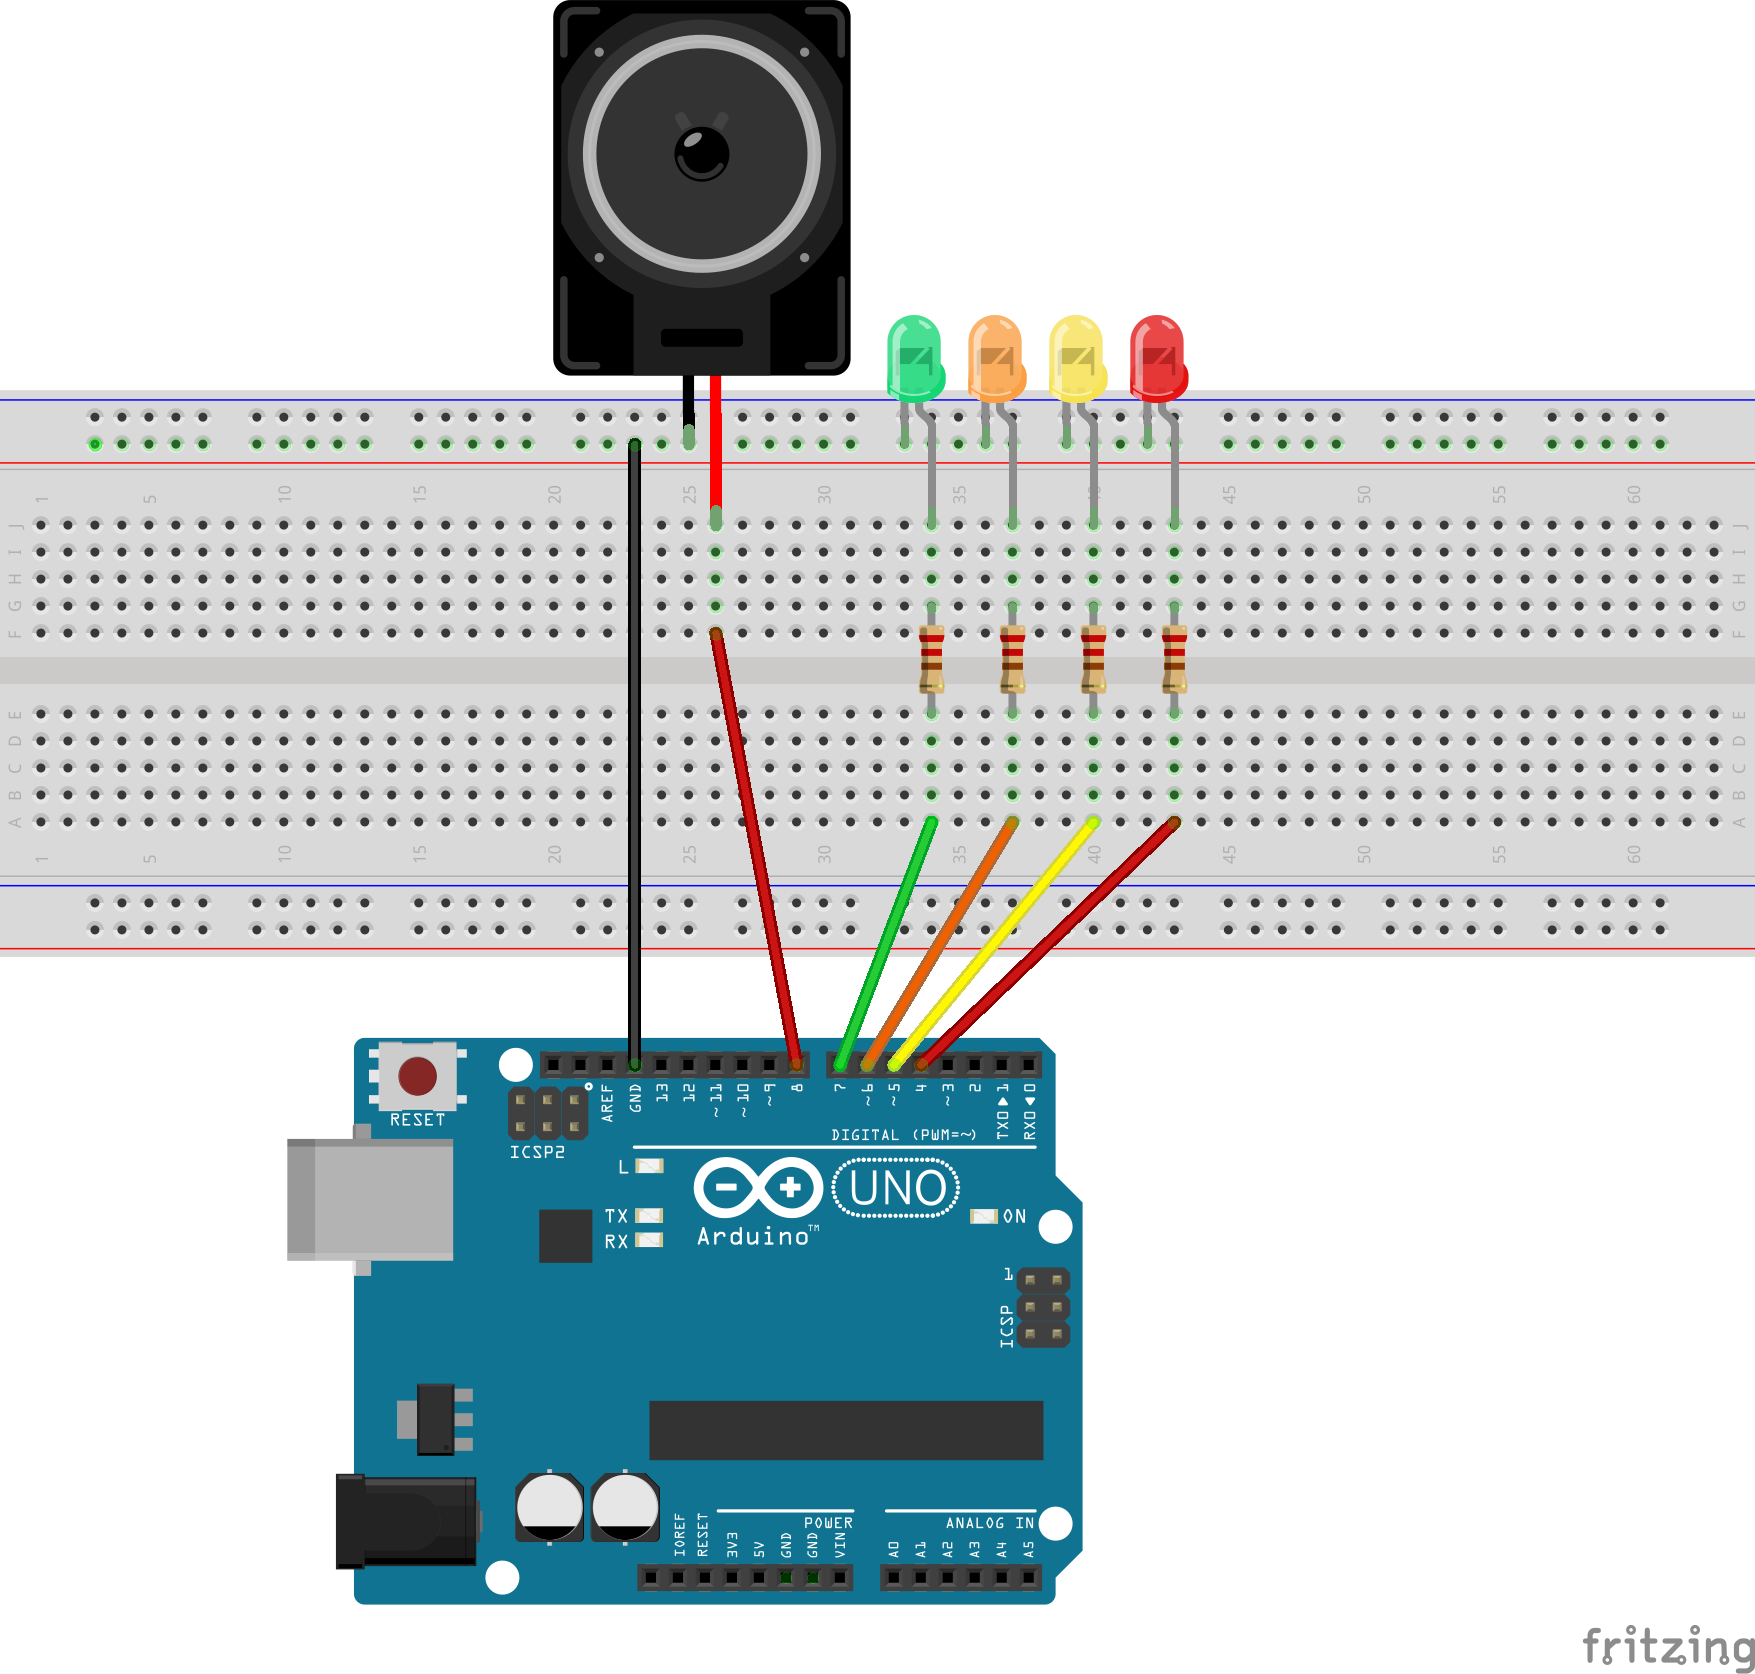
\includegraphics[scale=0.9]{images/schema_tests.png}
			\caption{Sch\'ema du prototype de test}
		\end{center}
	\end{figure}
	\begin{figure}
		\begin{center}
			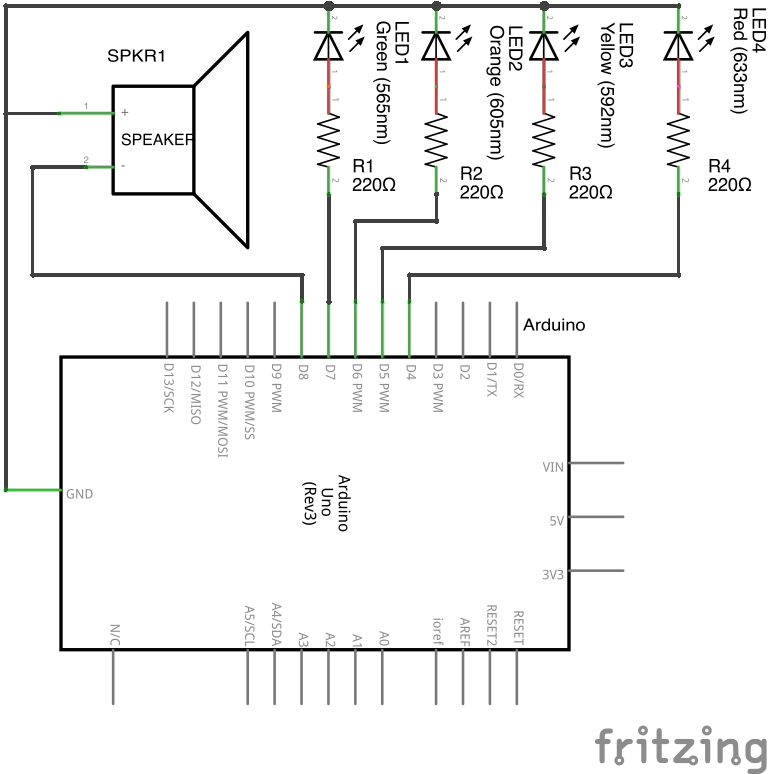
\includegraphics[scale=1]{images/schema_tests_elec.png}
			\caption{Sch\'ema \'electrique du prototype de test}
		\end{center}
	\end{figure}
\section{Tests finaux}
	%TODO
\section{Discussion et analyse}
\chapter*{Conclusion}
\appendix
	\chapter{Code des applications}
		%Modifications de l'affichage des codes source
		\lstset{
			numbers = left,
			showspaces = none,
			keepspaces = true,
			showstringspaces = true,
			basicstyle = \footnotesize,
			commentstyle = \color{newGreen},
			keywordstyle = \color{newOrange},
			identifierstyle = \color{newBlue},
			stringstyle = \color{newMauve}
		}
		\lstdefinestyle{arduino}{
			language=C,
			morekeywords = {HIGH, LOW, INPUT, OUTPUT}
		}
		\section{Application principale}
			\lstinputlisting[language=python]{../Application_finale/app.py}
		\section{Code Arduino pour les tests}
			\lstinputlisting[style=arduino]{../src/tests/tests.ino}
	%TODO~: bibliographie
\end{document}
